\documentclass{jarticle}
\usepackage{rsj}
\usepackage[dvips]{graphicx}
\usepackage{url}

\newcommand{\figref}[1]{\figurename\ref{fig:#1}}
\newcommand{\tabref}[1]{\tablename\ref{tab:#1}}

\begin{document}
\title{複数視点における画像意味分割の統合による三次元物体形状復元}
\author{和田健太郎, 48-166636}

\maketitle
% \thispagestyle{empty}
% \pagestyle{empty}

\begin{figure}[t]
  \centering
  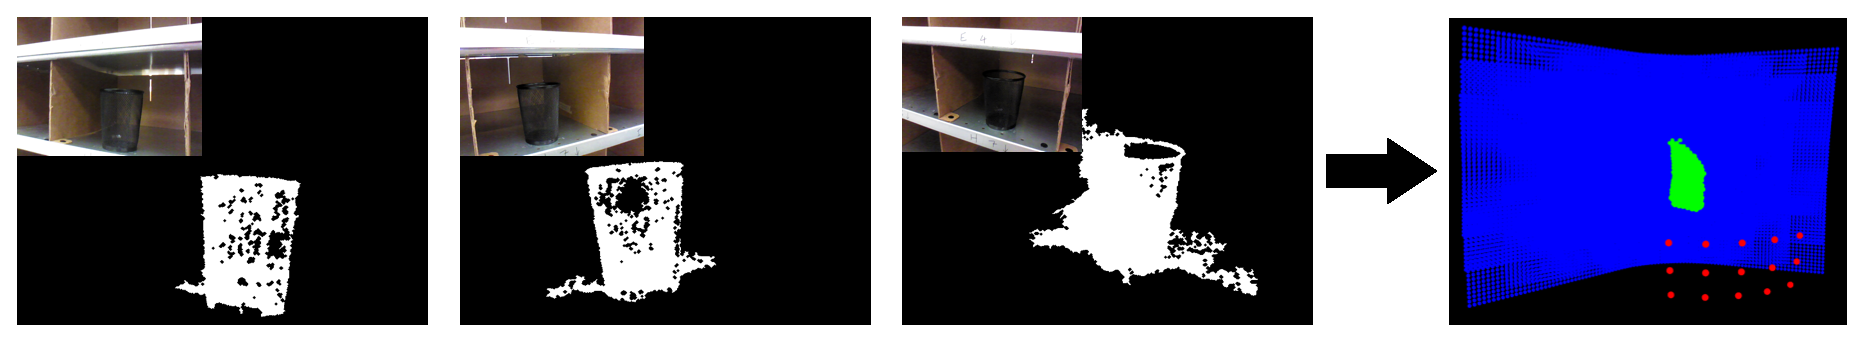
\includegraphics[width=\columnwidth]{figs/mask_fusion}
  \caption{三次元物体形状復元のパイプライン.}
  \label{fig:system}
\end{figure}

\section{序章}

三次元物体形状復元は現実世界における物体の三次元モデルを生成するもので,
ロボット\cite{eppner2016lessons}
や拡張現実\cite{newcombe2011kinectfusion}など三次元モデルを必要とするアプリケーションにおいて
必要な技術の一つである.
三次元モデルの必要とされる状況として,
整然とした環境においてモデルを生成(オフライン)と,
倉庫や家庭などの一般的な環境における生成(オンライン)とに大別できる.
後者の画像生成では物体の位置や背景が仮定できないという点で,
前者に比べより困難な問題設定になっていると言え、本レポートで取り組むこととする。

本レポートでは、オンラインでの生成において物体の意味分割と統合したシステムとして
形状復元を実現する。\ref{fig:system}が提案するシステムの概要図であり、
左側が色画像と物体意味分割結果によるマスク画像で、それらを統合することによって
右側のような三次元形状モデルを生成する。
右図において青がカメラフレームの遠方点、緑が物体形状、赤がカメラ視点を表す。
このシステムの入力となっているのは、色画像とマスク画像の他にカメラ視点
(ロボットがカメラを動かすこととする)
カメラパラメータ(キャリブレーション済みとする)がある。

提案手法はデプスや複数物体のマスク(ラベル画像)を複数視点で統合することができ、
\ref{fig:system}に示すようなデプス情報の取れない物体においても有効であることを示す。
実験はシステムの入力がペアとなった公開データセット\cite{zeng2016multi}を用いることによって行った。

\section{実験}

複数の画像での意味分割結果を統合するために、
本レポートでは立方体列(Voxel)を統合するためのフレームワークである
オクトマップ\cite{hornung2013octomap}を利用する。
カメラのマスクはカメラパラメータとカメラの位置情報によって三次元的な直線(Ray)として表すことができ、
このRayとVoxelとの交差を数えることによって複数視点での統合を行う。
ここでRayの長さがパラメータとなるが,実験では1mとした.
Rayの端点は\ref{fig:system}において青の点で示した.

さらにオンライン形状復元においては,複数の物体を同時に復元する必要がある.
そのため,マスク画像を複数物体に拡張したラベル画像を用いて,
各ラベルの値をカウントすることによって複数物体の同時形状復元を行う.
\ref{fig:label}にラベル画像を用いた同様のシステムを示す.
ラベル画像の色はそれぞれ別の物体クラスを表し,
複数物体においても同様に三次元復元ができていることがわかる.

\begin{figure}[htbp]
  \centering
  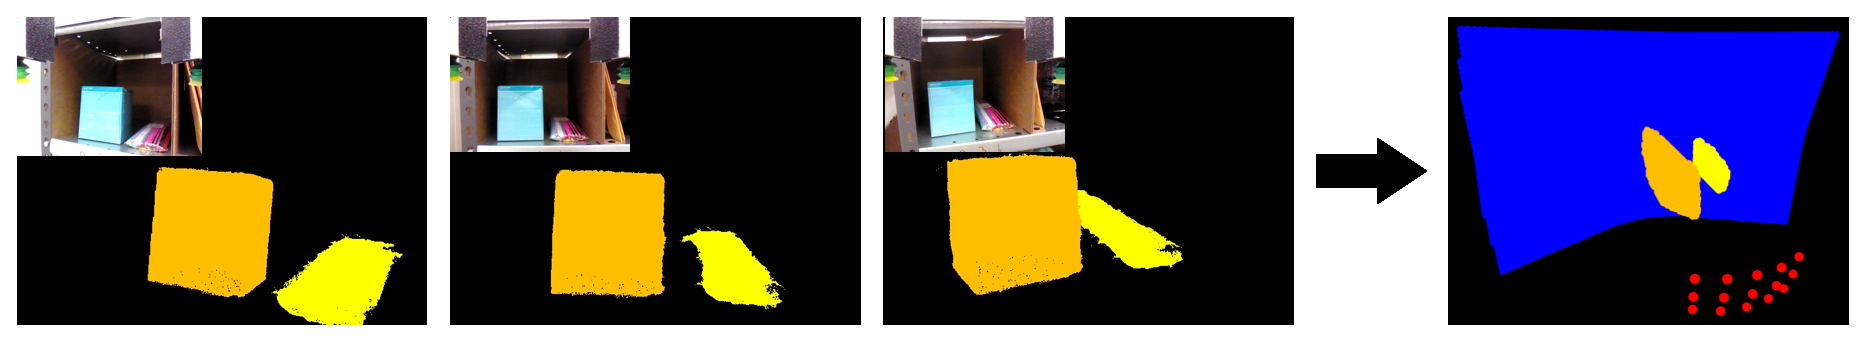
\includegraphics[width=\columnwidth]{figs/label_fusion}
  \caption{複数物体の形状復元.}
  \label{fig:label}
\end{figure}


\section{結論}

画像の意味分割とVoxelマッピングを統合することによって,
オンラインで三次元物体形状を生成することが可能であることを示した.
本レポートでは,講義で学習したカメラパラメータと環境の三次元点の関係と,
Voxelマッピング技術としてOctoMapというフレームワークを用いた.


{\footnotesize
%\small
\bibliographystyle{junsrt}
\bibliography{main}
}
\end{document}
